\chapter{Methodology}\label{ch: methodology}
This chapter covers the technical details of our experiment and analyses methodologies. We present our proposed target transformation technique Directional Change Transformation (DCT) in Section \ref{sec: dc transformation}. Then in Section \ref{sec: experiment}, we address the experiment we design to evaluate the transformation.

\section{DC Target Transformation}\label{sec: dc transformation}
Our proposed target transformation is called \textit{Directional Change (DC) Transformation}. The DC Transformation is a chain of operations to be embedded as the general target transformation procedure introduced in Section \ref{subsec: target transformation procedure}. Consider the general notation for a time series $\mathcal{Y}_{t_k} = \{y_{t_i}\}_{i = 1, 2, \ldots, k}$ and its timestamp set being $t$; for some mapping $X (\mathcal{Y}_{t_k}) = \mathcal{Y}^{(X)}_{t_k}$, we denote $y^{(X)}_{t_i}$ as an element in $\mathcal{Y}^{(X)}_{t_k}$ and $t^{(X)}$ being its timestamp set. Recall the log-difference transformation $\mathcal{T}^{(logr)}$ and DC algorithm $\mathcal{A}^{(DC)} (\cdot; \delta, \mathcal{R} (x; y))$ we addressed earlier. Then for an arbitrary model fitting to be conducted with time series $\mathcal{Y}_{t_k}$, DC Transformation goes as the following.

We start by performing the DC classification algorithm for a given $\delta$ and $\mathcal{R}$
\begin{equation*}
    \mathcal{Y}^{(DC)}_{t_k} = \mathcal{A}^{(DC)} (\mathcal{Y}_{t_k}; \delta, \mathcal{R} (x; y)).
\end{equation*}
We then collect the values marked as local extrema or confirmation of directional change events. Let $\mathcal{Y}^{(E)}_{t_k}$ be a subset of $\mathcal{Y}^{(DC)}_{t_k}$ such that
\begin{equation*}
    \mathcal{Y}^{(E)}_{t_k} = \{(y_{t_i}, s) | s = \text{local extreme} \vee \text{DC confirmation} \}_{t_i \in t}.
\end{equation*}
As $\mathcal{Y}^{(E)}_{t_k} \subset \mathcal{Y}^{(DC)}_{t_k}$, we look at the $y_{t_i}$ values in $\mathcal{Y}^{(E)}_{t_k}$ and perform interpolation for $t_i \in t - t^{(E)}$ to fill in the gaps between the event points in $\mathcal{Y}^{(E)}_{t_k}$. Note that the states $s$ assigned by $\mathcal{A}^{(DC)}$ are preserved and left unchanged because we are only operating on the values $y_{t_i}$. Let $\mathcal{I} (\mathcal{Y}^{(E)}_{t_k}, \mathcal{Y}^{(DC)}_{t_k})$ be an interpolation operation such that we have a new set given by
\begin{equation*}
    \mathcal{Y}^{(EI)}_{t_k} = \mathcal{I} (\mathcal{Y}^{(E)}_{t_k}, \mathcal{Y}^{(DC)}_{t_k}) = \begin{cases}
        (y_{t_i}, s)          &\text{if $t_i \in t - t^{(E)}$} \\
        (y^{(I)}_{t_i}, s)    &\text{otherwise}
    \end{cases}, \; \forall i \in \{1, 2, \cdots, k\}
\end{equation*}
where $y^{(I)}_{t_i}$ are the interpolated values generated by an interpolation $\mathcal{I}$. We note that after the interpolation, $\langle \mathcal{Y}^{(EI)}_{t_k} \rangle = \langle \mathcal{Y}_{t_k} \rangle$\footnote{Recall that we let $\langle \cdot \rangle$ be a counting operator of the number of elements in a finite set.}.

We visualise $\mathcal{Y}^{(EI)}_{t_k}$ and $\mathcal{Y}_{t_k}$ alongside with each other and with different $\delta$ and $\mathcal{I}$ settings to illustrate the effects. Let $\delta = (10\%, -10\%)$, $\mathcal{I}$ be a linear interpolation\footnote{If extrapolation is needed in the tail of the series, we simply leave the values unchanged.} and $\mathcal{R}$ be simple return as stated in Equation \ref{eq: return}, then we can have Figure \ref{fig: dct 10 linear}. The line in blue is $\mathcal{Y}_{t_k}$. The circles and diamonds mark the values in $\mathcal{Y}^{(E)}_{t_k}$. The line in green, along with the circles and diamonds, illustrates $\mathcal{Y}^{(EI)}_{t_k}$.
\begin{figure}[H]
    \centering
    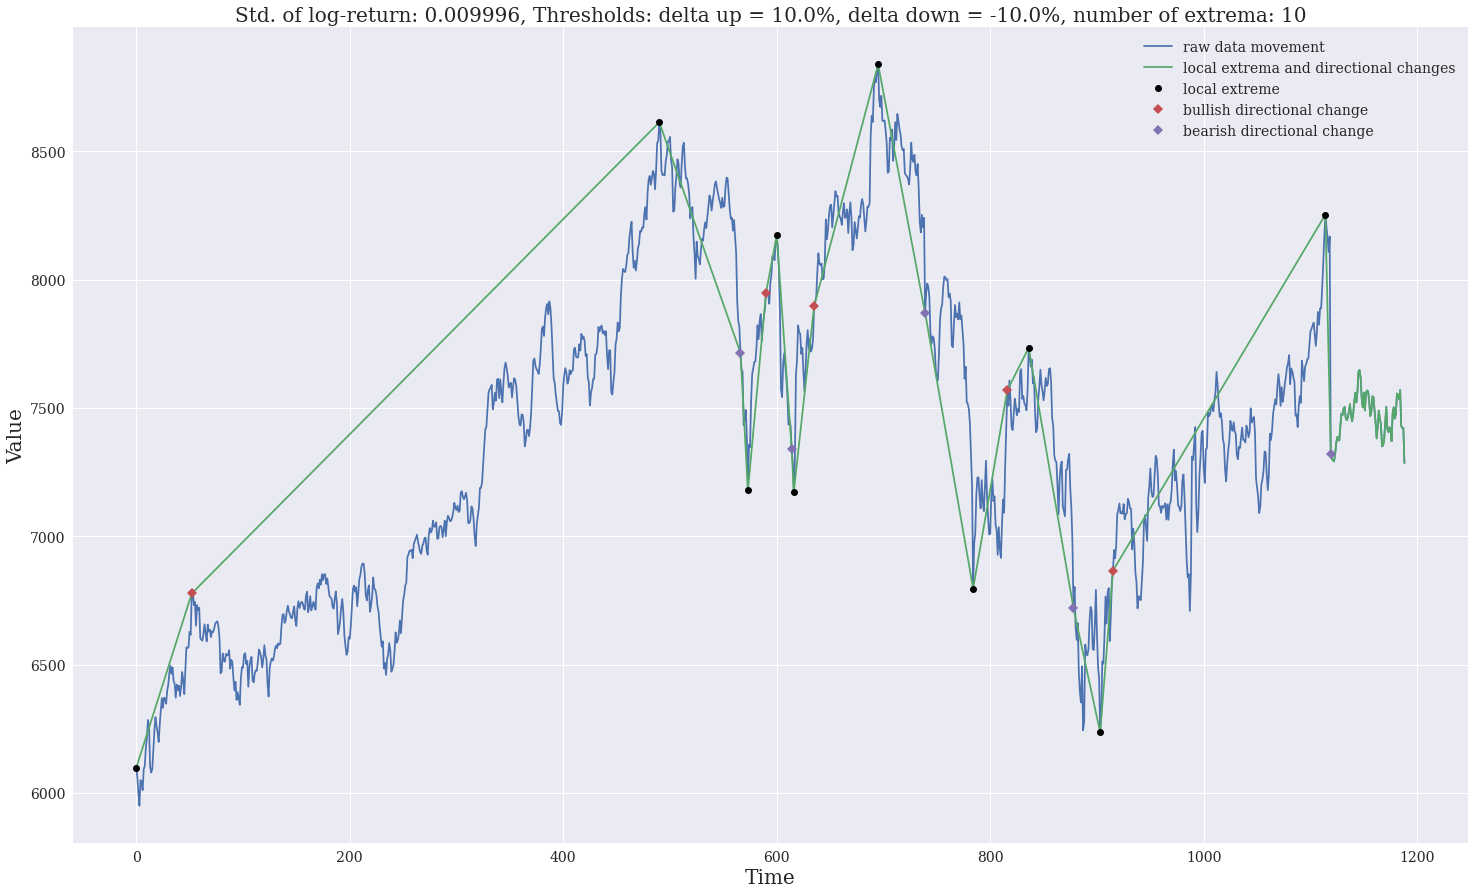
\includegraphics[width=\columnwidth]{DCT_10_linear}
    \caption{DC Transformed and original time series ($\delta = \pm 10\%$, linear)}
    {\raggedright \footnotesize \par}
    \label{fig: dct 10 linear}
\end{figure}
To observe the effect of different parameters, Figure \ref{fig: dct 5 linear} has a lower $\delta$ of $(5\%, -5\%)$. Decreasing the threshold values leads to the DC identification algorithm $\mathcal{A}^{(DC)}$ being more sensitive to events. We thus get a larger $\mathcal{Y}^{(E)}_{t_k}$ and narrower intervals to interpolate.
\begin{figure}[H]
    \centering
    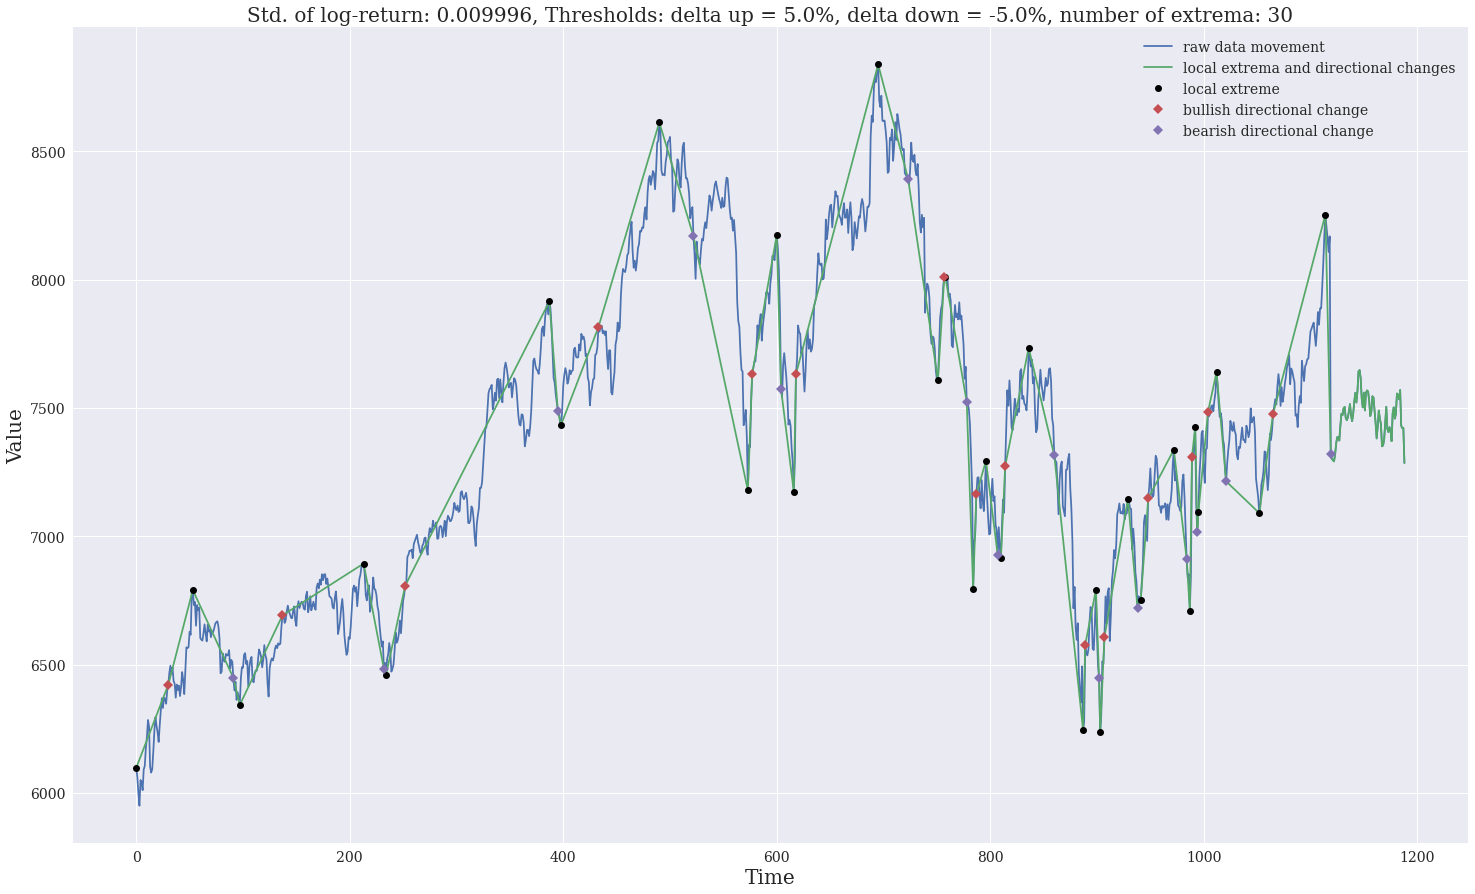
\includegraphics[width=\columnwidth]{DCT_5_linear}
    \caption{DC Transformed and original time series ($\delta = \pm 5\%$, linear)}
    {\raggedright \footnotesize \par}
    \label{fig: dct 5 linear}
\end{figure}
As to different interpolation methods, with Akima interpolation (Akima (\citeyear{akima1970new})), which is a variant of polynomial interpolation, we get what is shown in Figure \ref{fig: dct 5 akima}.
\begin{figure}[H]
    \centering
    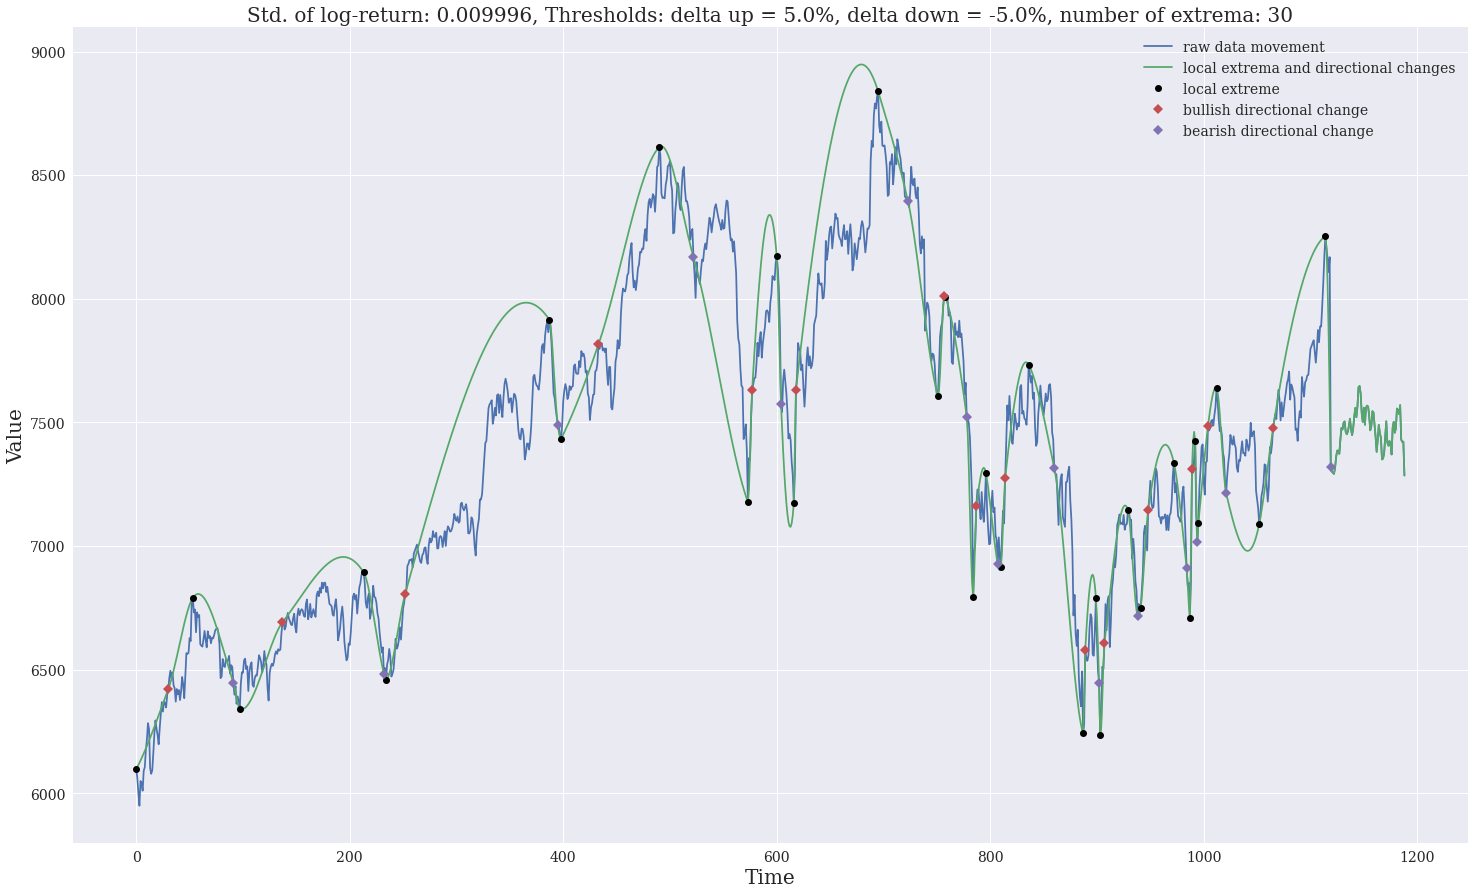
\includegraphics[width=\columnwidth]{DCT_5_akima}
    \caption{DC Transformed and original time series ($\delta = \pm 5\%$, akima)}
    {\raggedright \footnotesize \par}
    \label{fig: dct 5 akima}
\end{figure}

After having $\mathcal{Y}^{(EI)}_{t_k}$, we then apply the log-difference target transformation, which was introduced in Section \ref{subsec: log-diff transformation}. We get:
\begin{equation*}
    \mathcal{Y}^{(logrEI)}_{t_k} = \mathcal{T}^{(logr)}(\mathcal{Y}^{(EI)}_{t_k}) = \begin{cases}
        (\emptyset, s)  &\text{if $i = 1$} \\
        (\log(\frac{y^{(EI)}_{t_i}}{y_{t^{(EI)}_{i-1}}}), s) &\text{if $i = 2, 3, \cdots, k$}
    \end{cases}.
\end{equation*}
Figure \ref{fig: log-diff dct} demonstrates $\mathcal{Y}^{(logrEI)}_{t_k}$, which is the log-differenced $\mathcal{Y}^{(EI)}_{t_k}$.
\begin{figure}[H]
    \centering
    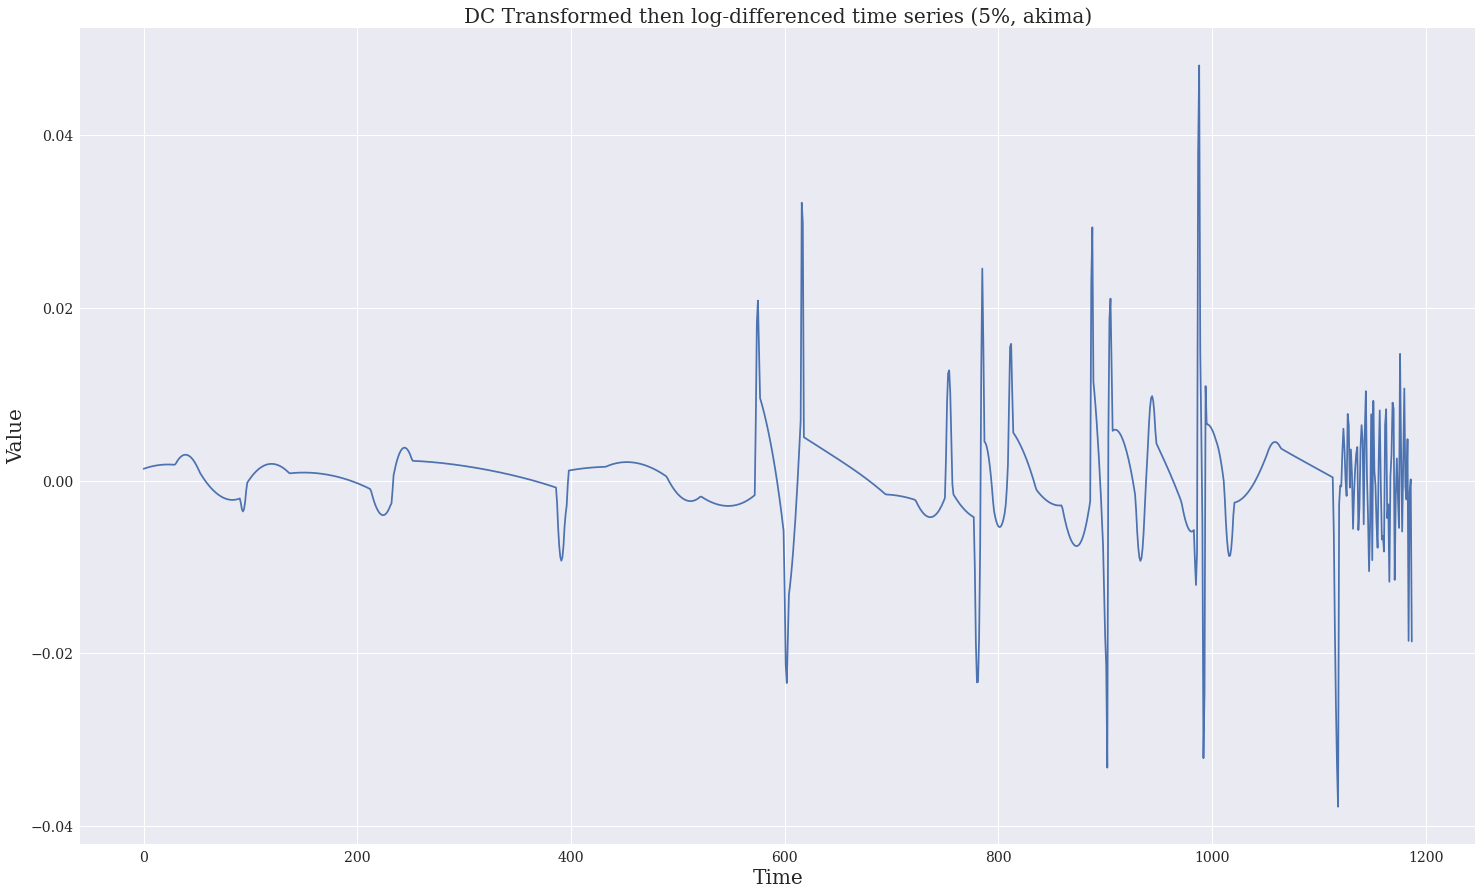
\includegraphics[width=\columnwidth]{log_diff_dct}
    \caption{DC Transformed then log-differenced time series ($\delta = \pm 5\%$, akima)}
    {\raggedright \footnotesize \par}
    \label{fig: log-diff dct}
\end{figure}

We can then generate the training target and design matrix with the $y^{(logrEI)}_{t_i}$ values in $\mathcal{Y}^{(logrEI)}_{t_k}$
\begin{gather*}
    \matr{y}^{(logrEI)}_{train}, \; \matr{X}^{(logrEI)}_{train} = \mathcal{S} (\mathcal{Y}^{(logrEI)}_{t_k} ; \tau, h=1, \lambda) \\
    \matr{y}^{(logrEI)}_{train} = \begin{bmatrix}
        y^{(logrEI)}_{t_\lambda}       \\
        y^{(logrEI)}_{t_{\lambda + 1}} \\
        \cdot               \\
        \cdot               \\
        y^{(logrEI)}_{t_{k-1}}         \\
        y^{(logrEI)}_{t_k}             \\
    \end{bmatrix}
    , \quad
    \matr{X}^{(logrEI)}_{train} = \begin{bmatrix}
        y^{(logrEI)}_{t_{\lambda} - \tau}   & y^{(logrEI)}_{t_{\lambda-1} - \tau} & \cdots & y^{(logrEI)}_{t_{1}} \\
        y^{(logrEI)}_{t_{\lambda+1} - \tau} & y^{(logrEI)}_{t_{\lambda} - \tau}   & \cdots & y^{(logrEI)}_{t_{2}} \\
        \cdot                    & \cdot                    & \cdots & \cdot     \\
        \cdot                    & \cdot                    & \cdots & \cdot     \\
        y^{(logrEI)}_{t_{k-1} - \tau}       & y^{(logrEI)}_{t_{k-2} - \tau}       & \cdots & y^{(logrEI)}_{t_{k - \lambda} - \tau}     \\
        y^{(logrEI)}_{t_{k} - \tau}         & y^{(logrEI)}_{t_{k-1} - \tau}       & \cdots & y^{(logrEI)}_{t_{k - \lambda + 1} - \tau} \\
    \end{bmatrix}.
\end{gather*}
Before fitting the model, we also introduce a feature generation method utilising the states produced by $\mathcal{A}^{(DC)}$. For each instance $y^{(logrEI)}_{t_i}$ in the training target $\matr{y}^{(logrEI)}_{train}$, we use the state $s$ of $y^{(logrEI)}_{t_i - \tau}$ from $\mathcal{Y}^{(logrEI)}_{t_k}$. Since $s$ is a categorical variable with seven possible outcomes as listed in Section \ref{subsec: dc algo}, it needs some further preprocessing to be suitable for predicting. We thus use \textit{one-hot encoding} for the categorical variable $s$. For $k - \lambda - 1$ predictions, we get a $k - \lambda - 1$ by seven matrix, where each row is the one-hot encoded vector of the corresponding $s$. We concatenate the one-hot encode matrix on the right side of $\matr{X}^{(logrEI)}_{train}$ and have a new design matrix $\matr{X}^{(SlogrEI)}$ with the one-hot encoded states.

We then fit the model with its loss function $\mathcal{E}$ to find the optimal parameter $\theta$ for the given hyperparameter $\phi_0$
\begin{equation*}
    \theta(\phi_0)_0 = \arg_{\theta(\phi_0)} \min \mathcal{E}(\widehat{\matr{y}}^{(SlogrEI)}_{train}, \matr{y}^{(logrEI)}_{train}), \; \widehat{\matr{y}}^{(SlogrEI)}_{train} = f(\theta(\phi_0); \matr{X}^{(SlogrEI)}_{train}).
\end{equation*}
After having the model, we make the input matrix also with the one-hot encoded state information and denote as\footnote{$\matr{X}^{(SlogrEI)}_{val}$ is of shape $1$ by the number of lags plus seven.}
\begin{equation*}
    \matr{X}^{(SlogrEI)}_{val}
\end{equation*}
and make a prediction using the trained model
\begin{equation*}
    \widehat{\matr{y}}^{(SlogrEI)}_{val} = f(\matr{X}^{(SlogrEI)}_{val} ; \theta(\phi_0)_0).
\end{equation*}
Obtain the validation target that we need for validation
\begin{equation*}
    \matr{y}_{val} = y_{t_k + \tau}.
\end{equation*}
Since the operations related to the DC framework do not contribute to the transformed prediction not being comparable to the original level, we only have to back-transform the change of scale introduced by log-differencing. Let the back transformation of log-differencing be denoted as $\mathcal{T}^{(b-logr)}$ and we have
\begin{equation*}
    \widehat{\matr{y}}^{(b-SlogrEI)}_{val} = \mathcal{T}^{(b-logr)} (\widehat{\matr{y}}^{(SlogrEI)}_{val} ; \mathcal{Y}_{t_k}).
\end{equation*}
Finally, we compute the validation score using the back-transformed prediction and the validation target by
\begin{equation*}
    \mathcal{V} (\widehat{\matr{y}}^{(b-SlogrEI)}_{val}, \matr{y}_{val}).
\end{equation*}
And that concludes the whole implementation of DC Transformation in a single model fitting. Then, as the stated standard modelling procedure, such a fitting process is repeated in the validation operation to compute the validation score for a single model setting (hyperparameter). Finally, we perform validation for all the hyperparameters and choose the one with the best validation score.

Let $\mathcal{T}^{(DC)}$ denotes the DC Transformation. $\mathcal{T}^{(DC)}$ is parameterised by the pair of threshold values $\theta$, the movement measure $\mathcal{R}$ and the interpolation method $\mathcal{I}$. As to back transformation, applying $\mathcal{T}^{(DC)}$ needs the log-differencing back transformation. In practice, all $\theta, \mathcal{R}$ and $\mathcal{I}$ can be explored during model selection. We can see that there are two components, each having different effects on the output: the DC algorithm $\mathcal{A}^{(DC)}$ captures the heads and tails of events while the interpolation component $\mathcal{I}$ creates a smooth process in between them. The threshold parameter $\delta$ controls the sensitivity of $\mathcal{A}^{(DC)}$ to events and thus affecting the number of intervals needed for interpolating and their width.

\section{Experiment}\label{sec: experiment}
This section discusses the experiment to investigate whether our proposed DC Transformation can positively affect univariate time series forecasting. The effectiveness of a target transformation technique depends on both the complementing model (the choice of $f$) and the dataset. To obtain robust and objective results, we experiment with different types of models that can be used for univariate time series forecasting and a large number of time series. In particular, we trained five models with and without DC Transformation over many time series and compared model performance.

\subsection{Dataset}
Our experiment's dataset is the one used in the M4 Competition (see Makridakis et al. \citeyear{MAKRIDAKIS202054}). It consists of 100,000 univariate time series with different frequencies and domains (see Table \ref{tbl: m4 dataset}). Although we intend to scale the experiment to have robust results, we cannot experiment on all the time series given our limited time. Therefore, we picked a subset of time series to experiment with. We intend to experiment on higher frequency and finance/economic related time series. We tested on a total of $458$ time series from the M4 dataset: $66$ of them are weekly financial time series, $252$ of them are daily time series from three different domains (Microeconomics, Macroeconomics, and Finance), and $140$ of them are hourly time series from an unknown domain (see Table \ref{tbl: ts used})\footnote{The time series in M4 dataset are indexed from $1$ to $100000$. We choose by their length: the daily and hourly time series chosen are the first in their domain with a length between $1000$ and $1500$; and the weekly financial time series chosen are the first to have a length between $600$ and $1500$.}.

\begin{center}
    \begin{table}
        \resizebox{\columnwidth}{!}{\begin{tabular}{| l || c c c c c c | r |} 
            \hline
            {}        & Micro & Industry & Macro & Finance & Demographic & Other & Total \\
            \hline\hline
            Yearly    & 6538 & 3716 & 3903 & 6519 & 1088 & 1236 & 23000 \\
            Quarterly & 6020 & 4637 & 5315 & 5305 & 1858 & 865  & 24000 \\
            Monthly   &10975 &10017 &10016 &10987 & 5728 & 277  & 48000 \\
            Weekly    & 112  & 6    & 41   & 164  & 24   & 12   & 359   \\
            Daily     & 1476 & 422  & 127  & 1559 & 10   & 633  & 4227  \\
            Hourly    & 0    & 0    & 0    & 0    & 0    & 414  & 414   \\
            \hline
            Total     &25121 &18798 &19402 &24534 & 8708 & 3437 & 100000 \\
            \hline
        \end{tabular}}
        \caption{Number of series in the M4 dataset per frequency and domain.}
        {\raggedright \footnotesize This table is a direct reference to the one in Makridakis et al. (\citeyear{MAKRIDAKIS202054}). \par}
        \label{tbl: m4 dataset}
    \end{table}
\end{center}

\begin{center}
    \begin{table}
        \centering
        \resizebox{0.7\columnwidth}{!}{\begin{tabular}{| l || c c c c | r |} 
            \hline
            {}        & Micro & Macro & Finance & Other & Total \\
            \hline\hline
            Weekly    & -     & -     & 66      & -     & 66  \\
            Daily     & 98    & 54    & 100     & -     & 252 \\
            Hourly    & -     & -     & -       & 140   & 140 \\
            \hline
            Total     & 98    & 60    & 166     & 140   & 458 \\
            \hline
        \end{tabular}}
        \caption{number of series used per frequency and domain.}
        {\raggedright \footnotesize \par}
        \label{tbl: ts used}
    \end{table}
\end{center}

\subsection{DC Transformation Settings}
Recall that DC Transformation is characterised by some parameters. For the movement measure $\mathcal{R} (x; y)$, we used the net return given by
\begin{equation*}
    \mathcal{R} (x; y) = \frac{x - y}{y}.
\end{equation*}
As to the interpolation method $\mathcal{I} (S_1, S_2)$ for two sets $S_1 \subset S_2$, we used a simple linear interpolation - the values in $S_1$ are connected with a straight line such that $\langle S_1 \rangle = \langle S_2 \rangle$. We did try other interpolation methods during exploratory trials. We will mention this in Chapter \ref{ch: results and eval}.

Regarding the most important parameter $\delta = (\delta_{down}, \delta_{up})$, we include this parameter into the hyperparameter set $\phi$ that has to be tuned. Since $\delta$ is correlated to the diffusion of the time series if considered as a stochastic process (see Appendix A in Petrov et al. (\citeyear{petrov2018agent})), the hyperparameter space is decided according to our simple estimation of the diffusion of the training time series if considered as a stochastic process. Let $\mathcal{Y}_{t_k}$ be an arbitrary training set, $\mathcal{T}^{(logr)}$ be the log-differencing operator described as Equation \ref{eq: log-differencing} in Section \ref{subsec: log-diff transformation} and $\text{Var}(\cdot)$ be the variance for a one-dimensional series excluding the empty values if there is any, then our estimation of the diffusion $\sigma$ is given by
\begin{align*}
    &\mathcal{Y}^{(logr)}_{t_k} = \mathcal{T}^{(logr)}(\mathcal{Y}_{t_k}) \\
    &\sigma = \sqrt{\text{Var}(\mathcal{Y}^{(logr)}_{t_k})}.
\end{align*}
The hyperparameter space of $\delta$ that we denoted as $H(\delta)$ is then based on the direct proportion of $\sigma$ and is given by\footnote{The operator `$\times$' between two finite sets is a cartesian product that gives all possible combinations of the elements in the two finite sets. For example, $\{a, b \} \times \{ 1, 2 \} = \{ (a, 1), (a, 2), (b, 1), (b, 2) \}$.}
\begin{gather*}
    A = \{ 0.01 \sigma, 0.21 \sigma, 0.41 \sigma, 0.61 \sigma, 0.81 \sigma, 1.01 \sigma, 1.21 \sigma, 1.41 \sigma, 1.61 \sigma, 1.81 \sigma, 2.01 \sigma \} \\
    H(\delta) = A \times A.
\end{gather*}
Observe that $H(\delta)$ is a set with $11 \times 11 = 121$ two-dimensional tuples. The first element in a tuple is the number for $\delta_{down}$ and the second for $\delta_{up}$.

\subsection{Models}\label{subsec: models}
This section covers the models we used and the hyperparameters we tuned in our experiment. The actual hyperparameter space we searched per model is provided in Appendix \ref{apdx: hyper space}. For the discussion in the rest of this section, consider an arbitrary training set $\mathcal{Y}_{t_k} = \{y_{t_i} \}_{i = 1, 2, \ldots, k}$ and its corresponding $\matr{y}$ and $\matr{X}$ derived from $\mathcal{S}$ be target and design matrix with $n$ rows (instances), $\phi$ as the hyperparameter set, and $\theta$ the parameter set for the model.

\subsubsection{Elastic Net Regression Model}
We use Elastic Net (EN) as our representative for linear regression methodologies. EN can be written as
\begin{gather*}
    f^{(EN)} (\matr{X} ; \theta = (\matr{w}, \matr{\beta})) = \matr{X} \matr{w} + \matr{\beta} = \widehat{\matr{y}}.
\end{gather*}
The structure and determination of $\theta$ is controlled by hyperparameters $\phi = (l, \alpha, \rho)$ and the optimisation
\begin{equation*}
    \theta_{best} = \arg_{\theta} \min \frac{1}{2n} L_2(\matr{X} \matr{w} + \matr{\beta} - \matr{y}) + \alpha \rho L_1(\matr{w}) + \frac{\alpha (1 - \rho)}{2} L_2(\matr{w})
\end{equation*}
where
\begin{itemize}
    \item $n$ is the number of training instances, i.e., the length of $\matr{y}$,
    \item $l$ is the number of lags. As mentioned in Section \ref{subsec: ML modelling}, the bigger $l$ is, the more past information the model is allowed to use for a single prediction. $l$ also affects the length of the weight vector $\matr{w}$.
    \item $\alpha > 0, \; \alpha \in \mathbb{R}$ is the regularisation constant determining the scale of the penalty.
    \item $L_1$ and $L_2$ are L1 and L2 norm respectively.
    \item $\rho \in [0, 1]$ is the weight assigned to $L_1$ penalty.
\end{itemize}

\subsubsection{Multilayer Perceptron Regressor}
To have a non-linear regression model, we chose the Multilayer Perceptron (MLP) regressor. MLP is controlled by $\phi = (l, strucs, max iter)$ where
\begin{itemize}
    \item $l$ is the number of lags,
    \item $strucs$ is a tuple. Element number $i$ in $stucs$ determines the number of hidden neurons in hidden layer $i$. For example, $strucs = (5, 10)$ means the MLP has two hidden layers, with the first having five hidden neurons and the second having ten.
    \item $max iter$ is the maximum iterations the solver is allowed to go through.
\end{itemize}
Every neuron in the MLP model is a linear combination of an input vector. $neuron: \mathbb{R}^m \longmapsto \mathbb{R}$. Depending on the dimension of the input, i.e., $m$, a neuron is parameterised by a $m$ dimension weight vector. These neurons form a neural network, which is a non-linear function of the input vector. The weights are trained using a variant of stochastic gradient descent solver (see Kingma et al. \citeyear{kingma2014adam}).

\subsubsection{Linear Support Vector Regressor}
Linear Support Vector Regressor (LSVR) is a member of the \textit{Kernel Methods} that uses a linear kernel. We chose LSVR for its faster implementation than typical SVR with other kernels. LSVR is parameterised by $\theta = (\matr{w}, \matr{b})$ much like a linear regression model
\begin{equation*}
    f^{(LSVR)} (\matr{X} ; \theta = (\matr{w}, \matr{b})) = \matr{X} \matr{w} + \matr{b} = \widehat{\matr{y}}.
\end{equation*}
where $\theta$ is decided by solving the optimisation problem
\begin{equation*}
    \theta_{best} = \arg_{\theta = (\matr{w}, \matr{b})} \min (\frac{1}{2} L_2(\matr{w}) + C \sum_{i=1}^{n} \max(0, |\matr{y}_i - (\matr{w}^T I(\matr{X}_i) + \matr{b})| - \epsilon))
\end{equation*}
where
\begin{itemize}
    \item $L_2$ is the L2 norm.
    \item $I$ is the identity function.
    \item $\epsilon$ characterises the \textit{Vapnik's $\epsilon$-insensitive loss function} that makes a `tube' with radius $\epsilon$ around the target $\matr{y}$. The decision of this value should depend on the scale of $\matr{y}$. We have it defaulted to $0$ as suggested by \href{https://scikit-learn.org/stable/modules/generated/sklearn.svm.LinearSVR.html#sklearn.svm.LinearSVR}{scikit learn}.
\end{itemize}
The hyperparameter set characterising the decision of $\theta$ we tune is $\phi = (l, tol, C)$ where
\begin{itemize}
    \item $l$ is the number of lags,
    \item $tol$ is the tolerance for the stopping condition during the,
    \item $C$ is the regularisation constant similar to $\alpha$ for EN. However, by the implementation, $C$ is inversely proportional to the strength of the penalty.
\end{itemize}

\subsubsection{Random Forest Regressor}
Our representative for tree-based models is Random Forest Regressor (RF) because it trains faster than other tree-based methods, such as Gradient Boosting Machine or Light Gradient Boosting Machine. RF is an ensemble method that applies \textit{Bootstrap Aggregation (Bagging)} method on both the training instances and the features. In other words, the trees in the ensemble are trained on different training instances and features. Bagging on features is applied randomly. Such a method is called the \textit{random subspace method}. The hyperparameter set we tuned is $\phi = (l, min sample split)$ where
\begin{itemize}
    \item $l$ is the number of lags.
    \item $min sample split$ sets the minimum number of samples required to split an existing node. The value is positively correlated to the strength of pruning as a regularisation measure.
\end{itemize}
The parameter $\theta$ is a combination of decision criteria of the decision trees in the ensemble.

\subsubsection{Exponential Smoothing Forecasting Model}
Exponential Smoothing (ETS) is not a regression model, as in, it does not estimate its parameters with our target $\matr{y}$ and design matrix $\matr{X}$ environment. ETS trains directly on the univariate time series $\mathcal{Y}_{t_k} = \{ y_{t_i}\}_{i = 1, 2, \ldots, k}$. ETS has many variants. The one we used here is based on the implementation of \href{https://www.rdocumentation.org/packages/forecast/versions/8.12/topics/ets}{R Version of ETS} (see Hyndman et al. \citeyear{hyndman2008admissible} and Hyndman et al. \citeyear{hyndman2008forecasting}). This version of ETS implicitly tunes the hyperparameter $\phi = (trend, seasonal, damped)$ where
\begin{itemize}
    \item $seasonal \in \{ \text{additive}, \text{multiplicative} \}$ is a binary variable setting whether the seasonal component in the model is additive or multiplicative. An additive seasonal component fits better when there is not much seasonal variation, while a multiplicative seasonal component is made for the cases where seasonal variation is proportional to the level of the time series.
    \item $trend \in \{ \text{additive}, \text{multiplicative} \}$ is a binary variable setting whether the trend component in the model is additive or multiplicative.
    \item $damped \in \{ \text{True}, \text{False} \}$ is a binary variable setting whether the damped trend methods is applied. The damped trend method dampens the trend component to a constant into the future to prevent the model from over-forecasting for future values.
\end{itemize}
ETS essentially uses a weighted average of the past observations as its prediction. In the sense that a weighted average is a form of linear combination, ETS is much like EN according to how we train it. $\theta$ is a vector of weights assigned to the past observations ETS uses for its prediction.

\begin{comment}
    \subsubsection{Moving Average}
    A simple Moving Average (MA) model is used as a benchmark. MA is simple an average of the past observations. The number of past observations used for the averaging is parameterised by $\theta = (q)$. Note that for $q = 1$, if MA is a \textit{naive forecasting} - MA uses the latest observation as its prediction.
\end{comment}
\subsection{Agent}
For each model we mentioned in the previous section, we train the model with and without applying DC Transformation on the set of time series we chose from the M4 dataset. As a result, we end up having ten agents
\begin{equation*}
    \{\text{EN}, \text{MLP}, \text{LSVR}, \text{RF}, \text{ETS} \} \times \{ \text{with DC Transform}, \text{without DC Transform} \}
\end{equation*}
each being trained on many time series.

\subsection{Performance Metrics}\label{subsec: performance metrics}
We consult the experiment described in Ahmed et al. (\citeyear{2010EmpiricalMLComparison}) for our performance metrics. Our main performance measure is the Symmetric Mean Absolute Percentage Error (SMAPE)\footnote{This is also the main error measure for M3 Competition (see Makridak et al. \citeyear{makridakis2000m3})}. For a single prediction $\widehat{\matr{y}}_i \in \widehat{\matr{y}}$ and the target $\matr{y}_i \in \matr{y}$, the Symmetric Absolute Percentage Error (SAPE) is given by
\begin{equation*}
    SAPE(\widehat{\matr{y}}_i, \matr{y}_i) = \frac{2| \widehat{\matr{y}}_i - \matr{y}_i|}{|\widehat{\matr{y}}_i| + |\matr{y}_i| }
\end{equation*}
where the operator $| \cdot |$ is the norm of a vector (can be L1, L2 or others). However, seeing that our forecasting horizon is fixed to one for all forecasting tasks, we have $\widehat{\matr{y}}_i, \matr{y}_i \in \mathbb{R}$. So we can see $| \cdot |$ as the absolute operator of a real number. Then for a set of $m$ validation or testing points, SMAPE is given by
\begin{equation*}\label{eq: smape}
    SMAPE(\widehat{\matr{y}}, \matr{y}) = \frac{1}{m} \sum_{i=1}^{m} \frac{2| \widehat{\matr{y}}_i - \matr{y}_i|}{|\widehat{\matr{y}}_i| + |\matr{y}_i| }
\end{equation*}
Observe that SMAPE is scale-free because it is a relative error measure. We can combine the SMAPE yielded from different time series with different scales. This is one of the main reasons we chose SMAPE as our primary error measure.

We also calculate a ranking measure as a summary statistics. Let $Q=10$ be the total number of agents. For a time series, we have $Q$ agents trained and their corresponding SMAPE scores. We rank these $Q$ agents based on their SMAPE - the agent with the lowest SMAPE is ranked number one, the largest the last. For $P$ time series that all $Q$ agents have been trained on, an agent has $P$ ranks. Let $R_{q, p}$ denote the rank of model $q$ on time series $p$. We have a distribution of ranks for an agent $q$ and can calculate the mean given by
\begin{equation*}\label{eq: rank}
    R_q = \frac{1}{P} \sum_{p = 1}^{P}R_{q, p}.
\end{equation*}
Moreover, treating $R_q$ as a random variable, we can come up with a confidence interval for the ranking of an agent $q$. Let $c_{\alpha, Q}$ be the upper $\alpha$ percentile of the range for $Q$ independent standard Gaussian normal variables. Then the $\alpha$ percent confidence interval of the ranking for agent $q$ is given by
\begin{equation*}\label{eq: rank interval}
    R_q \pm 0.5 c_{\alpha, Q} \sqrt{\frac{Q(Q+1)}{12 P}}.
\end{equation*}
See Koning et al. (\citeyear{KONING2005397}) for further details of such statistics.

Another summary performance measure we calculated is called the `fraction-best' measure (see Section Five in Ahmed et al. (\citeyear{2010EmpiricalMLComparison})). The fraction-best is also a rank-based measure. It measures how often an agent ranks top-performing out of all $P$ time series tested. That is, if agent $q$ is ranked number one for $n$ times out of $P$ time series, the fraction-best for agent $q$ is given by
\begin{equation*}\label{eq: frac best}
    FB_q = \frac{n}{P}.
\end{equation*}
There could be occasions where an agent is conditionally performant, i.e., an agent is particularly good only under limited circumstances. In such cases, the agent can have a mediocre average SMAPE score but an impressive fraction-best score. Calculating the fraction-best score helps identify such agents if they exist.

\subsection{Modelling configuration}
In this section, we present some other configurations for our experiment. All agents use log-differencing as their basic target transformation method during the model fitting. Log-differencing helps make the time series stationary. The validation size $v$ and test size $\kappa$ are fixed to ten percent of the length of the training set size for all time series. We treat the time series as time-homogeneous, i.e., the values in a time series are indexed by the nature number set sequentially. The forecast horizon is fixed to one, and the gap is fixed to one step for all forecasting objectives. As to the retrain window, we have different retrain window sizes for time series with different frequencies. For hourly, daily and weekly frequencies, we have a retrain window of ten, i.e., the model updates its parameters every ten steps. For monthly frequency, we have a retrain window of size six; this means that the model parameters get updated every six steps. Since the goal of our experiment is to compare how models perform with and without the DC Transformation, the retrain window should not affect our conclusions: all agents compete under the same conditions.
